\documentclass[12pt]{article}
\usepackage{{../preamble}}
\graphicspath{{pics}}

\begin{document}
\chead{Problem Set 2}

%%%%%%%%%%%%%%%%%%%%%%%%%%%%%%%%%%%%%%%%%%%%%%%
%                  Definitions                %
%%%%%%%%%%%%%%%%%%%%%%%%%%%%%%%%%%%%%%%%%%%%%%%
\def\xdot{\dot X} \def\ydot{\dot Y} \def\zdot{\dot Z}
\def\kdot{\dot k} \def\ccdot{\dot c} \def\ddt{\frac{d}{dt}}
\def\dfdk{\frac{\partial F}{\partial K}}
\def\dfdl{\frac{\partial F}{\partial L}}
\def\plim{\lim\limits_{\phi\to 0}}
\def\ddp{\dfrac{\partial}{\partial \phi}}
\def\dgdp{\dfrac{\partial\gamma}{\partial \phi}}
\def\invphi{\sfrac{1}{\phi}}




%%%%%%%%%%%%%%%%%%%%%%%%%%%%%%%%%%%%%%%%%%%%%%%
%                Problem 1                    %
%%%%%%%%%%%%%%%%%%%%%%%%%%%%%%%%%%%%%%%%%%%%%%%
\section*{Problem 1}
\problem{Growth, saving, and $r-g$: Romer 2.6}{
    Piketty (2014) argues that a fall in the growth rate
of the economy is likely to lead to an increase in the difference between the real
interest rate and the growth rate. This problem asks you to investigate this issue
in the context of the Ramsey Cass Koopmans model. Specifically, consider a
Ramsey Cass Koopmans economy that is on its balanced growth path, and suppose
there is a permanent fall in $g$.

    \begin{enumerate}[label=(\alph*)]
    \item How, if at all, does this affect the $\kdot = 0$ curve?
    \end{enumerate} 
}


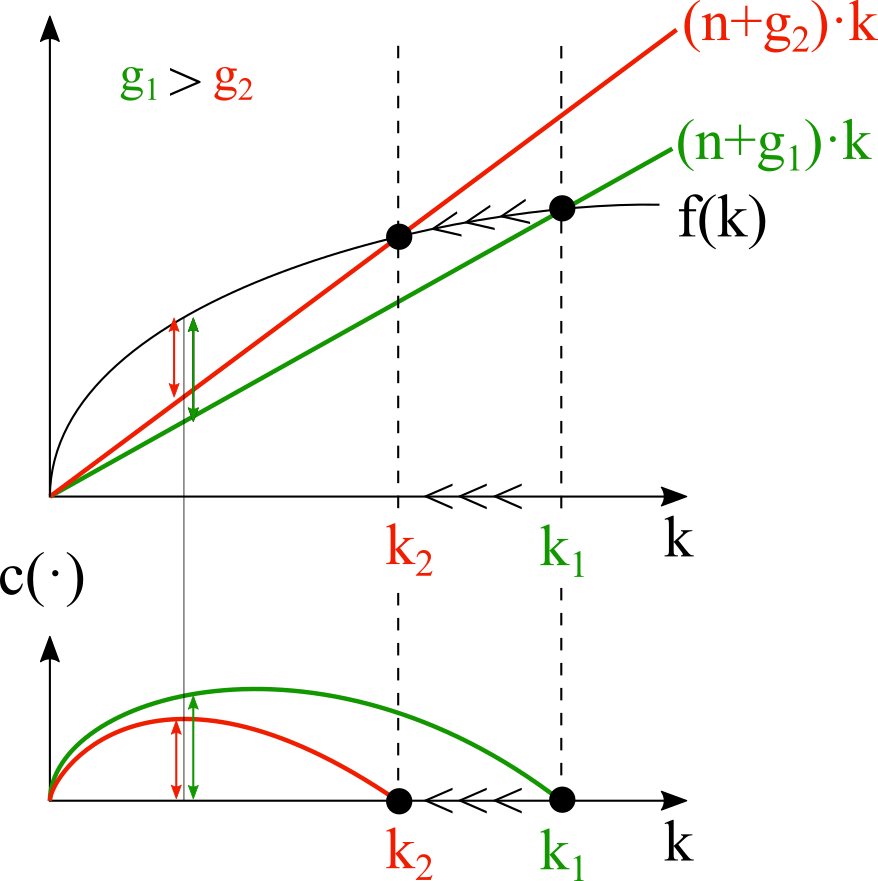
\includegraphics[width=0.5\textwidth]{1.a}


In the plot above, we can see a decrease in $g$
\begin{itemize}
    \item[$\implies$] a decrease in the slope of $(n+g)k$
    \item[$\implies$] increase in the $k$ where $f(k)-(n+g)k=0$
    \item[$\implies$] increase in the $k$ where the $\kdot=0$ curve meets the $k$ axis
\end{itemize}

A decrease in the slope of $(n+g)k$ also implies that the distance between $(n+g)k$ and $f(k)$ will be larger $\forall k$ between 0 and where $f(k)-(n+g)k=0$.

\noindent
So, overall, a decrease in $g$ implies a vertical and horizontal stretch outward for the $\kdot = 0$ curve.


%%%%%%%%%%%%%%%%%
%     Part b    %
%%%%%%%%%%%%%%%%%
\newpage\problem{}{
    \begin{enumerate}[label=(\alph*)]
    \setcounter{enumi}{1}
    \item How, if at all, does this affect the $\ccdot = 0$ curve?
    \end{enumerate} 
}


%%%%%%%%%%%%%%%%%
%     Part c    %
%%%%%%%%%%%%%%%%%
\newpage\problem{}{
    \begin{enumerate}[label=(\alph*)]
    \setcounter{enumi}{2}
    \item At the time of the change, does $c$ rise, fall, or stay the same, or is it not possible to tell?
    \end{enumerate} 
}


%%%%%%%%%%%%%%%%%
%     Part d    %
%%%%%%%%%%%%%%%%%
\newpage\problem{}{
    \begin{enumerate}[label=(\alph*)]
    \setcounter{enumi}{3}
    \item At the time of the change, does $r-g$ rise, fall, or stay the same, or is it not possible to tell?
    \end{enumerate} 
}


%%%%%%%%%%%%%%%%%
%     Part e    %
%%%%%%%%%%%%%%%%%
\newpage\problem{}{
    \begin{enumerate}[label=(\alph*)]
    \setcounter{enumi}{4}
    \item In the long run, does $r-g$ rise, fall, or stay the same, or is it not possible to tell?
    \end{enumerate} 
}


%%%%%%%%%%%%%%%%%
%     Part f    %
%%%%%%%%%%%%%%%%%
\newpage\problem{}{
    \begin{enumerate}[label=(\alph*)]
    \setcounter{enumi}{5}
    \item Find an expression for the impact of a marginal change in $g$ on the fraction of output that is saved on the balanced growth path. Can one tell whether this expression is positive or negative?
    \end{enumerate} 
}


%%%%%%%%%%%%%%%%%
%     Part g    %
%%%%%%%%%%%%%%%%%
\newpage\problem{}{
    \begin{enumerate}[label=(\alph*)]
    \setcounter{enumi}{6}
    \item For the case where the production function is Cobb-Douglas, $f'(k^*) = k^\alpha$, rewrite your answer to part (f) in terms of $\rho, n, g, \theta,$ and $\alpha$. (Hint: Use the fact that $f'(k^*) = \rho + \theta g$.)
    \end{enumerate} 
}



%%%%%%%%%%%%%%%%%%%%%%%%%%%%%%%%%%%%%%%%%%%%%%%
%                Problem 2                    %
%%%%%%%%%%%%%%%%%%%%%%%%%%%%%%%%%%%%%%%%%%%%%%%
\newpage
\section*{Problem 2}
\problem{Capital taxation in the Ramsey-Cass-Koopmans model: Romer 2.10}{
    Consider a Ramsey-Cass-Koopmans economy that is on its balanced growth path. Suppose
that at some time, which we will call time 0, the government switches to a policy
of taxing investment income at rate $\tau$. Thus the real interest rate that households
face is now given by \[r(t) = (1-\tau) f'(k(t)).\] Assume that the government returns
the revenue it collects from this tax through lump-sum transfers. Finally, assume
that this change in tax policy is unanticipated.

    \begin{enumerate}[label=(\alph*)]
    \item How, if at all, does the tax affect the $\ccdot = 0$ locus? The $\kdot = 0$ locus?
    \end{enumerate} 
}



%%%%%%%%%%%%%%%%%
%     Part b    %
%%%%%%%%%%%%%%%%%
\newpage\problem{}{
    \begin{enumerate}[label=(\alph*)]
    \setcounter{enumi}{1}
    \item How does the economy respond to the adoption of the tax at time 0? What are the dynamics after time 0?
    \end{enumerate} 
}


%%%%%%%%%%%%%%%%%
%     Part c    %
%%%%%%%%%%%%%%%%%
\newpage\problem{}{
    \begin{enumerate}[label=(\alph*)]
    \setcounter{enumi}{2}
    \item How do the values of $c$ and $k$ on the new balanced growth path compare with their values on the old balanced growth path?
    \end{enumerate} 
}


%%%%%%%%%%%%%%%%%
%     Part d    %
%%%%%%%%%%%%%%%%%
\newpage\problem{}{
    \begin{enumerate}[label=(\alph*)]
    \setcounter{enumi}{3}
    \item (This is based on Barro, Mankiw, and Sala-i-Martin, 1995.) Suppose there are many economies like this one. Workers’ preferences are the same in each country, but the tax rates on investment income may vary across countries. Assume that each country is on its balanced growth path.
    
    \begin{enumerate}[label=(i)]
        \item Show that the saving rate on the balanced growth path, $(y^* - c^*)/y^*$, is decreasing in $\tau$.
    \end{enumerate}
    \end{enumerate} 
}



%%%%%%%%%%%%
% Part ii %
%%%%%%%%%%%
\newpage\problem{}{
    \begin{enumerate}[label=(ii)]
    \item Do citizens in low-$\tau$, high-$k^*$, high-saving countries have any incentive to invest in low-saving countries? Why or why not?
    \end{enumerate} 
}



%%%%%%%%%%%%%%%%%
%     Part e    %
%%%%%%%%%%%%%%%%%
\newpage\problem{}{
    \begin{enumerate}[label=(\alph*)]
    \setcounter{enumi}{4}
    \item Does your answer to part (c) imply that a policy of \textit{subsidizing} investment (that is, making $\tau<0$), and raising the revenue for this subsidy through lump-sum taxes, increases welfare? Why or why not?
    \end{enumerate} 
}


%%%%%%%%%%%%%%%%%
%     Part f    %
%%%%%%%%%%%%%%%%%
\newpage\problem{}{
    \begin{enumerate}[label=(\alph*)]
    \setcounter{enumi}{5}
    \item How, if at all, do the answers to parts (a) and (b) change if the government does not rebate the revenue from the tax but instead uses it to make government purchases?
    \end{enumerate} 
}





\end{document}

